\documentclass[12pt]{article}
\usepackage[left=1cm, right=1cm, top=2cm,bottom=1.5cm]{geometry} 

\usepackage[parfill]{parskip}
\usepackage[utf8]{inputenc}
\usepackage[T2A]{fontenc}
\usepackage[russian]{babel}
\usepackage{enumitem}
\usepackage[normalem]{ulem}
\usepackage{amsfonts, amsmath, amsthm, amssymb, mathtools}

\usepackage{tabularx}
\usepackage{hhline}

\usepackage{accents}
\usepackage{fancyhdr}
\pagestyle{fancy}
\renewcommand{\headrulewidth}{1.5pt}
\renewcommand{\footrulewidth}{1pt}

\usepackage{graphicx}
\usepackage[figurename=Рис.]{caption}
\usepackage{subcaption}
\usepackage{float}

%%Наименование папки откуда забирать изображения
\graphicspath{ {./images/} }

%%Изменение формата для ввода доказательства
\renewcommand{\proofname}{$\square$  \nopunct}
\renewcommand\qedsymbol{$\blacksquare$}

%%Изменение отступа на таблицах
\addto\captionsrussian{%
	\renewcommand{\proofname}{$\square$ \nopunct}%
}
%% Римские цифры
\newcommand{\RN}[1]{%
	\textup{\uppercase\expandafter{\romannumeral#1}}%
}

%% Для удобства записи
\newcommand{\MR}{\mathbb{R}}
\newcommand{\MC}{\mathbb{C}}
\newcommand{\MQ}{\mathbb{Q}}
\newcommand{\MN}{\mathbb{N}}
\newcommand{\MZ}{\mathbb{Z}}
\newcommand{\MTB}{\mathbb{T}}
\newcommand{\MTI}{\mathbb{I}}
\newcommand{\MI}{\mathrm{I}}
\newcommand{\MJ}{\mathrm{J}}
\newcommand{\MH}{\mathrm{H}}
\newcommand{\MT}{\mathrm{T}}
\newcommand{\MU}{\mathcal{U}}
\newcommand{\MV}{\mathcal{V}}
\newcommand{\MB}{\mathcal{B}}
\newcommand{\MW}{\mathcal{W}}
\newcommand{\ML}{\mathcal{L}}
\newcommand{\MP}{\mathcal{P}}
\newcommand{\VN}{\varnothing}
\newcommand{\VE}{\varepsilon}

\theoremstyle{definition}
\newtheorem{defn}{Опр:}
\newtheorem{rem}{Rm:}
\newtheorem{prop}{Утв.}
\newtheorem{exrc}{Упр.}
\newtheorem{lemma}{Лемма}
\newtheorem{theorem}{Теорема}
\newtheorem{corollary}{Следствие}

\newenvironment{cusdefn}[1]
{\renewcommand\thedefn{#1}\defn}
{\enddefn}

\DeclareRobustCommand{\divby}{%
	\mathrel{\text{\vbox{\baselineskip.65ex\lineskiplimit0pt\hbox{.}\hbox{.}\hbox{.}}}}%
}
%Короткий минус
\DeclareMathSymbol{\SMN}{\mathbin}{AMSa}{"39}
%Длинная шапка
\newcommand{\overbar}[1]{\mkern 1.5mu\overline{\mkern-1.5mu#1\mkern-1.5mu}\mkern 1.5mu}
%Функция знака
\DeclareMathOperator{\sgn}{sgn}

%Функция ранга
\DeclareMathOperator{\rk}{\text{rk}}

%Обозначение константы
\DeclareMathOperator{\const}{\text{const}}

\DeclareMathOperator*{\dsum}{\displaystyle\sum}
\newcommand{\ddsum}[2]{\displaystyle\sum\limits_{#1}^{#2}}

%Интеграл в большом формате
\DeclareMathOperator{\dint}{\displaystyle\int}
\newcommand{\ddint}[2]{\displaystyle\int\limits_{#1}^{#2}}
\newcommand{\ssum}[1]{\displaystyle \sum\limits_{n=1}^{\infty}{#1}_n}

\newcommand{\smallerrel}[1]{\mathrel{\mathpalette\smallerrelaux{#1}}}
\newcommand{\smallerrelaux}[2]{\raisebox{.1ex}{\scalebox{.75}{$#1#2$}}}

\newcommand{\smallin}{\smallerrel{\in}}
\newcommand{\smallnotin}{\smallerrel{\notin}}

\newcommand*{\medcap}{\mathbin{\scalebox{1.25}{\ensuremath{\cap}}}}%
\newcommand*{\medcup}{\mathbin{\scalebox{1.25}{\ensuremath{\cup}}}}%

\makeatletter
\newcommand{\vast}{\bBigg@{3.5}}
\newcommand{\Vast}{\bBigg@{5}}
\makeatother

%Промежуточное значение для sup\inf, поскольку они имеют разную высоту
\newcommand{\newsup}{\mathop{\smash{\mathrm{sup}}}}
\newcommand{\newinf}{\mathop{\mathrm{inf}\vphantom{\mathrm{sup}}}}

%Скалярное произведение
\newcommand{\inner}[2]{\left\langle #1, #2 \right\rangle }

%Подпись символов снизу
\newcommand{\ubar}[1]{\underaccent{\bar}{#1}}

%% Шапка для букв сверху
\newcommand{\wte}[1]{\widetilde{#1}}

%%Взятие в скобки, модули и норму
\newcommand{\parfit}[1]{\left( #1 \right)}
\newcommand{\modfit}[1]{\left| #1 \right|}
\newcommand{\sqparfit}[1]{\left\{ #1 \right\}}
\newcommand{\normfit}[1]{\left\| #1 \right\|}

%%Функция для обозначения равномерной сходимости по множеству
\newcommand{\uconv}[1]{\overset{#1}{\rightrightarrows}}
\newcommand{\uconvm}[2]{\overset{#1}{\underset{#2}{\rightrightarrows}}}


%%Функция для обозначения нижнего и верхнего интегралов
\def\upint{\mathchoice%
	{\mkern13mu\overline{\vphantom{\intop}\mkern7mu}\mkern-20mu}%
	{\mkern7mu\overline{\vphantom{\intop}\mkern7mu}\mkern-14mu}%
	{\mkern7mu\overline{\vphantom{\intop}\mkern7mu}\mkern-14mu}%
	{\mkern7mu\overline{\vphantom{\intop}\mkern7mu}\mkern-14mu}%
	\int}
\def\lowint{\mkern3mu\underline{\vphantom{\intop}\mkern7mu}\mkern-10mu\int}


\begin{document}
\lhead{Математический анализ - \RN{3}}
\chead{Шапошников С.В.}
\rhead{Лекция - 28}
\section*{Поточечная сходимость тригонометрического ряда Фурье}

\begin{prop}
	Набор функций: 
	$$
		\left\{\dfrac{1}{\sqrt{2\pi}}, \, \dfrac{\cos{nx}}{\sqrt{\pi}}, \, \dfrac{\sin{nx}}{\sqrt{\pi}}  \biggm\vert  n \in \MN  \right\}
	$$ 
	является полной ортонормированной системой в пространстве $R[0,2\pi]$.
\end{prop}

\begin{corollary}
	$\forall f \in R[0,2\pi]$ раскладывается в ряд Фурье по системе: $
	\left\{\dfrac{1}{\sqrt{2\pi}}, \, \dfrac{\cos{nx}}{\sqrt{\pi}}, \, \dfrac{\sin{nx}}{\sqrt{\pi}}  \biggm\vert  n \in \MN  \right\}
	$.
\end{corollary}

\begin{defn}
	\uwave{Тригонометрическим рядом Фурье} функции $f \in R[0,2\pi]$ называют функциональный ряд вида:
	$$
		f(x) = \dfrac{a_0}{2} + \ddsum{n = 1}{\infty}\left(a_n \cos{(nx)} + b_n \sin{(nx)}\right)
	$$
	$$
		a_n = \dfrac{1}{\pi}\ddint{0}{2\pi}f(t)\cos{(nt)}dt, \, \forall n \in \MN
	$$
	$$	
		b_n = \dfrac{1}{\pi}\ddint{0}{2\pi}f(t)\sin{(nt)}dt, \, \forall n \in \MN
	$$
\end{defn}

Мы остановились на том, что понимаем под равенством выше сходимость в виде:
$$
	\sqrt{\ddint{0}{2\pi} \left|f(x) -   \left(\dfrac{a_0}{2} + \ddsum{n = 1}{N}\left(a_n \cos{(nx)} + b_n \sin{(nx)}\right)\right) \right|^2 dx} = \sqrt{\ddint{0}{2\pi}\left| f(x) - S_N(x) \right|^2dx} \xrightarrow[N \to \infty]{} 0
$$
Заметим, что из сходимости в среднеквадратическом смысле (в виде интеграла) не следует сходимость почти всюду или вообще в каждой точке. Тем не менее, есть теорема Л'Карлесона ($1966$): 
$$
	\forall f \in R[0,2\pi], \, S_N \to f \text{ почти всюду}
$$
то есть, сходимость есть для всех точек $x$ кроме точек меры ноль. Перед нами стоит следующий вопрос, когда будет выполнено поточечное равенство? В каких-то точках будет сходиться или нет? Если возьмем некоторую точку $x$, можно ли утверждать что при некоторых условиях равенство $f(x)$ тригонометрическому ряду Фурье понимается в обычном смысле?

\begin{lemma}(\textbf{Римана})
	Если $f \in R[a,b]$, то: $\lim\limits_{\lambda \to \infty}\ddint{a}{b}f(x)\cos{(\lambda x)}dx =0$, $\lim\limits_{\lambda \to \infty}\ddint{a}{b}f(x)\sin{(\lambda x)}dx =0$.
\end{lemma}
\begin{proof}
	Возьмем промежуток $\{c,d\} \subset [a,b]$, пусть для начала $f = \MTI_{\{c,d\}}$, тогда:
	$$
		\ddint{a}{b}f(x)\cos{(\lambda x)}dx = \ddint{c}{d}\cos{(\lambda x)}dx = \dfrac{\sin{\lambda d} - \sin{\lambda c}}{\lambda} \xrightarrow[\lambda \to \infty]{} 0
	$$
	Аналогично для интеграла с синусом. Пусть $f_{\MTB}(x)$ это функция из утверждения о полноте тригонометрической системы по отрезку $[a,b]$:
	$$
		f_{\MTB}(x) = \ddsum{k = 1}{N}\inf\limits_{\Delta_k}f{\cdot}\MTI_{\Delta_k}(x)
	$$
	Оценим разность между исходной функцией $f(x)$ и $f_{\MTB}(x)$:
	$$
		\left|\ddint{a}{b}f(x)\cos{(\lambda x)}dx - \ddint{a}{b}f_{\MTB}(x)\cos{(\lambda x)}dx \right| \leq \ddint{a}{b}|f(x) - f_{\MTB}(x)|{\cdot}1 \, dx =  \ddint{a}{b}|f(x) - f_{\MTB}(x)| dx
	$$
	Пользуясь выводом из того же утверждения, мы получим:
	$$
		\forall \VE > 0, \, \exists \, f_{\MTB} \colon \ddint{a}{b}|f(x) - f_{\MTB}(x)| dx < \VE
	$$
	Фиксируем разбиение $\MTB$, тогда:
	$$
		\left|\ddint{a}{b}f(x)\cos{(\lambda x)}dx \right| =  
		\left|\ddint{a}{b}f(x)\cos{(\lambda x)}dx - \ddint{a}{b}f_{\MTB}(x)\cos{(\lambda x)}dx + \ddint{a}{b}f_{\MTB}(x)\cos{(\lambda x)}dx \right| \leq 
	$$
	$$	
		\ddint{a}{b}|f(x) - f_{\MTB}(x)| dx + \left|\ddint{a}{b}f_{\MTB}(x)\cos{(\lambda x)}dx \right|	
		\leq \VE + \left|\ddint{a}{b}f_{\MTB}(x)\cos{(\lambda x)}dx \right| \xrightarrow[\lambda \to \infty]{} \VE + 0 = \VE \Rightarrow
	$$
	$$
		\Rightarrow \exists \, \lambda_0 \colon \forall \lambda > \lambda_0, \, \left|\ddint{a}{b}f_{\MTB}(x)\cos{(\lambda x)}dx \right| < \VE \Rightarrow 	\left|\ddint{a}{b}f(x)dx \right| < 2\VE
	$$
	
\end{proof}
\begin{rem}
	Попробуем понять неформальное объяснение леммы. 
	\begin{figure}[H]
		\centering
		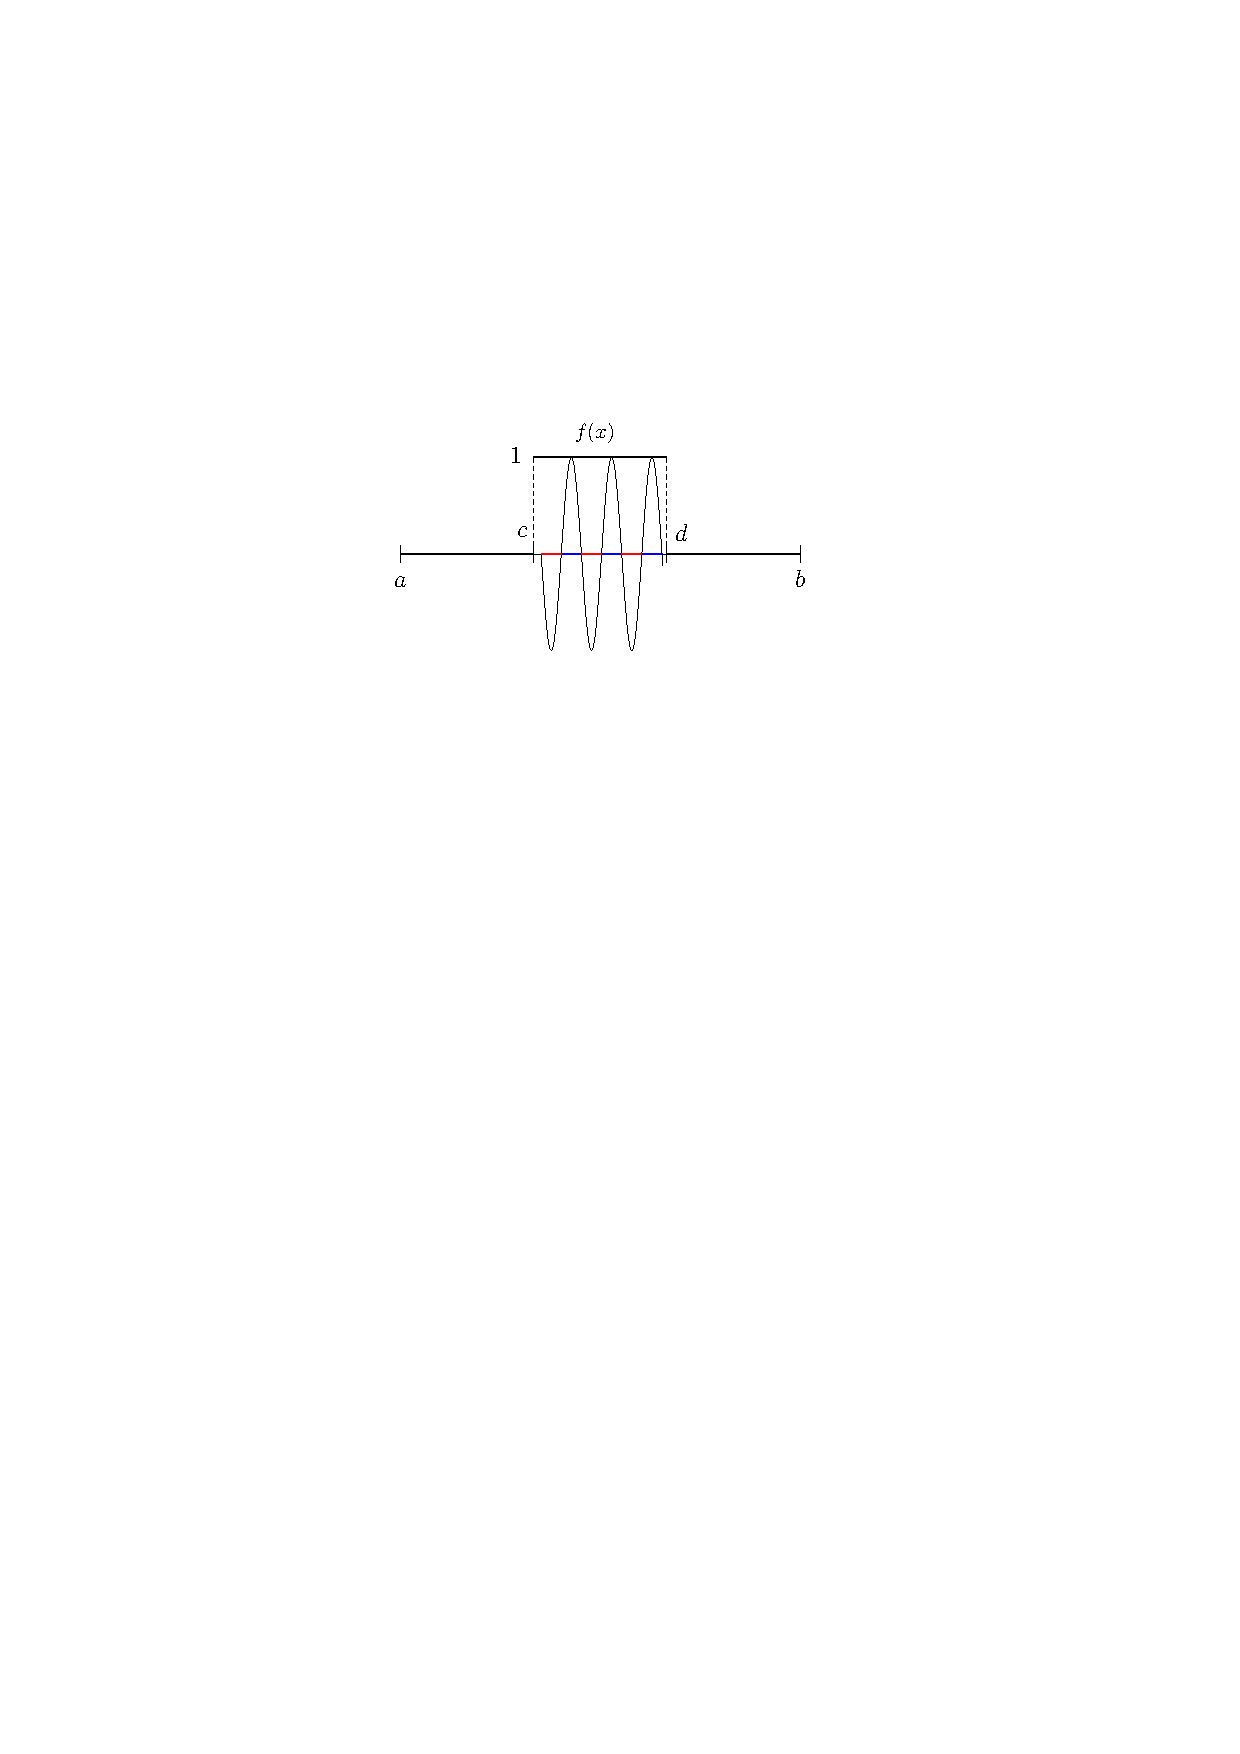
\includegraphics[width=0.35\textwidth]{MA3L28_1.png}
		\label{MA3L28_1}
		\caption{Поведение произведения индикаторной функции $f(x) =\MTI_{\{c,d\}}(x)$ и $\cos{\lambda x}$.}
		\label{fig: Построение функции}
	\end{figure}
	На отрезке $[a,b]$ имеем ступеньку на промежутке $\{c,d\}$ и на этом промежутке начинаем рисовать $\cos{\lambda x}$. При устремлении $\lambda$ в бесконечность, косинус начнет очень быстро колебаться $\Rightarrow$ за исключением отрезков рядом с точками $c$ и $d$ будет интегрирование косинуса по периоду (число красных промежутков на рисунке равно числу синих промежутков за исключением интервалов на концах), поэтому этот интеграл сокращается. Как мы уже выясняли, любая функция из $R[a,b]$ приближается такими ступенчатыми функциями и на каждом интервале происходит сокращение. 
\end{rem}

\newpage
\subsection*{Ядро Дирихле}
Чтобы продвинуться дальше в понимании сходимости, попробуем понять, как устроены частичные суммы тригонометрического ряда Фурье:
$$
	S_N(x) =\dfrac{a_0}{2} + \ddsum{n = 1}{N}\left(a_n \cos{nx} + b_n \sin{nx}\right) =
\dfrac{1}{2}{\cdot}\dfrac{1}{\pi}\ddint{0}{2\pi}f(t)dt + 
$$
$$
	+ \ddsum{n = 1}{N}\left(\dfrac{1}{\pi}\ddint{0}{2\pi}f(t){\cdot}\left(\cos{nt}\cos{nx} + \sin{nt}\sin{nx}\right)dt\right) 
	=	\dfrac{1}{\pi}\ddint{0}{2\pi}f(t){\cdot}\left(\dfrac{1}{2} + \ddsum{n = 1}{N}\cos{n(x-t)}\right)dt
$$
\begin{defn}
	\uwave{Ядром Дирихле} назовем следующую функцию: $D_N(t) = 1 + 2\left(\cos{t} + \cos{2t} + \dotsc + \cos{Nt}\right)$.
\end{defn}
Таким образом, мы можем переписать частичную сумму:
$$
	S_N(x) = \dfrac{1}{2\pi}\ddint{0}{2\pi}f(t)D_N(x -t)dt
$$
Несложно увидеть в полученном свёртку. Пусть $f \in R[0,2\pi]$ и продолжена как $2\pi$-периодическая функция и далее везде будем так считать, тогда у нас будет свёртка двух $2\pi$-периодических функций:
$$
	S_N(x) = \dfrac{1}{2\pi}f*D_N(x)
$$
Когда эта свёртка сходится к $f$? Как мы уже знаем, $S_N(x)$ сходится к $f(x)$, когда $D_N(x)$ - дельтаобразная последовательность. Тем самым возникает вопрос о том, как устроено ядро Дирихле.

\begin{theorem}(\textbf{свойства ядра Дирихле})
	\begin{enumerate}[label=\arabic*)]
		\item $D_N$ - гладкая $2\pi$-периодическая и четная функция;
		\item $\dfrac{1}{2\pi}\ddint{0}{2\pi} D_N(t)dt = 1$;
		\item $D_N(t) = 
			\left\{
			\begin{array}{rl}
				2N + 1, & t = 2\pi m \\[5pt]
				\dfrac{\sin{(N + \frac{1}{2})t}}{\sin{\frac{t}{2}}}, & t \neq 2\pi m
			\end{array}\right.$;
		\item $\forall \delta \in (0,\pi), \, \ddint{\delta}{2\pi - \delta}D_N(t)dt = 2\ddint{\delta}{\pi}D_N(t)dt \xrightarrow[N \to \infty]{} 0$;
	\end{enumerate}
\end{theorem}
\begin{rem}
	Для того, чтобы объявить ядро Дирихле дельтаобразной последовательностью нехватает неотрицательности и этим свойством ядро как раз не обладает. Более того, свойства ядра следуют из-за знакопеременности (увидим, что следуют из леммы Римана). Более того, важное $4)$-ое свойство как раз следует из осцилируемости ядра и поставив модуль уже будет не верно.
\end{rem}
\newpage
\begin{proof}\hfill
	\begin{enumerate}[label=\arabic*)]
		\item По определению функция Дирихле это конечная линейная комбинация косинусов и константы $\Rightarrow$ гладкая, $2\pi$-периодическая из-за косинусов, четная также из-за косинусов;
		\item $\dfrac{1}{2\pi}\ddint{0}{2\pi}D_N(t)dt = \dfrac{1}{2\pi}\ddint{0}{2\pi}dt + 2\dfrac{1}{2\pi}\ddint{0}{2\pi}\left(\cos{t} + \cos{2t} + \dotsc + \cos{Nt}\right)dt = \dfrac{2\pi}{2\pi} + 0 = 1$;
		\item Если $t = 2\pi n$, то $D_N(t) = 1 + \underbrace{2{\cdot}1 + 2{\cdot}1 + \dotsc + 2{\cdot}1}_{N} = 1 + 2N$. 
		
		Если $t \neq 2\pi n$, то домножим $D_N(t)$ на $\sin{\tfrac{t}{2}}$:
		$$
			D_N(t)\sin{\tfrac{t}{2}} = \sin{\tfrac{t}{2}} + 2 \sin{\tfrac{t}{2}}\cos{t} + \dotsc + 2\sin{\tfrac{t}{2}}\cos{Nt} = \sin{\tfrac{t}{2}} - \sin{\tfrac{t}{2}} + \sin{\tfrac{3t}{2}} - \sin{\tfrac{3t}{2}} + \dotsc +
		$$
		$$
			+ \sin{\left(N - \tfrac{1}{2}\right)t} - \sin{\left(N - \tfrac{1}{2}\right)t} + \sin{\left(N + \tfrac{1}{2}\right)t} \Rightarrow D_N(t) = \dfrac{\sin{\left(N + \tfrac{1}{2}\right)t}}{\sin{\tfrac{t}{2}}}
		$$
		где мы воспользовались следующим:
		$$
			2\sin{\tfrac{t}{2}}\cos{kt} = \sin{\left(\left(k + \tfrac{1}{2}\right)t\right) } - \sin{\left(\left(k -\tfrac{1}{2}\right)t\right)}
		$$
		
		\item Возьмем $\delta \in (0,\pi)$ и рассмотрим интеграл:
		$$
			\ddint{\delta}{2\pi - \delta}D_N(t)dt = \ddint{\delta}{\pi}D_N(t)dt + \ddint{\pi}{2\pi - \delta}D_N(t)dt = \ddint{\delta}{\pi}D_N(t)dt + \ddint{-\pi}{ - \delta}D_N(t)dt =
		$$
		$$
			= \ddint{\delta}{\pi}D_N(t)dt - \ddint{-\pi}{ - \delta}D_N(-t)d(-t) = \ddint{\delta}{\pi}D_N(t)dt - \ddint{\pi}{\delta}D_N(s)ds = 2\ddint{\delta}{\pi}D_N(t)dt
		$$
		где мы воспользовались периодичностью и четностью ядра Дирихле. Распишем интеграл явно, поскольку $t \neq 2\pi n$ на отрезке $[\delta,\pi]$, то:
		$$
			2\ddint{\delta}{\pi}D_N(t)dt = 2 \ddint{\delta}{\pi}\dfrac{1}{\sin{\tfrac{t}{2}}}{\cdot}\sin{\left(N + \tfrac{1}{2}\right)t}\,dt
		$$
		Заметим, что $\dfrac{1}{\sin{\tfrac{t}{2}}} \in C[\delta,\pi] \Rightarrow \dfrac{1}{\sin{\tfrac{t}{2}}} \in R[\delta,\pi]$, а $\sin{\left(N + \tfrac{1}{2}\right)t} = \sin{\lambda t}$, таким образом мы можем\\[4pt] применить лемму Римана:
		$$
			2 \ddint{\delta}{\pi}\dfrac{1}{\sin{\tfrac{t}{2}}}{\cdot}\sin{\left(N + \tfrac{1}{2}\right)t}\,dt \xrightarrow[N\to  \infty]{} 0
		$$
	\end{enumerate}
\end{proof}
\newpage
Перепишем частичные суммы ряда Фурье в более удобном виде:
$$
	S_N(x) = \dfrac{1}{2\pi}\ddint{0}{2\pi}f(t)D_N(x-t)dt = f* D_N(t) = D_N *f(t) = \dfrac{1}{2\pi}\ddint{0}{2\pi}f(x-t)D_N(t)dt =
$$
$$
	= \dfrac{1}{2\pi}\left(\ddint{0}{\pi}f(x-t)D_N(t)d + \ddint{\pi}{2\pi}f(x-t)D_N(t)dt  \right) = \dfrac{1}{2\pi}\left(\ddint{0}{\pi}f(x-t)D_N(t)d + \ddint{-\pi}{0}f(x-t)D_N(t)dt  \right)
$$
где последнее равенство выполнено в силу периодичности $D_N(t)$. Сделаем замену $t \to -t$:
$$
	\dfrac{1}{2\pi}\left(\ddint{0}{\pi}f(x-t)D_N(t)d + \ddint{-\pi}{0}f(x-t)D_N(t)dt  \right) = \dfrac{1}{2\pi}\left(\ddint{0}{\pi}f(x-t)D_N(t)d + \ddint{0}{\pi}f(x + s)D_N(s)ds  \right) =
$$
$$
	= \dfrac{1}{2\pi}\ddint{0}{\pi}(f(x - t) + f(x + t))D_N(t)dt 
$$

\begin{theorem}(\textbf{принцип локализации Римана})
	Пусть $f,g \in R[0,2\pi]$, $2\pi$-периодические и $f = g$ в окрестности точки $x_0: \MU(x_0)$, тогда ряды Фурье $f$ и $g$ сходятся и расходятся в точке $x_0$ одновременно и в случае сходимости их суммы совпадают.
\end{theorem}
\begin{rem}
	Отметим, что коэффициенты Фурье вычисляются на всём отрезке $[0,2\pi]$, а оказывается, что для сходимости в конкретной точке это всё неважно. Важно лишь то, как ведёт себя функция рядом с точкой $x_0$ и совершенно неважно, как ведёт себя функция вне этой окрестности.
\end{rem}
\begin{proof}
	Рассмотрим частичные суммы в точке $x_0$. Пусть $\delta > 0$ таково, что $f =g$ на $(x_0 - \delta, x_0 + \delta)$, тогда:
	$$
		S_N^f(x_0) = \dfrac{1}{2\pi}\ddint{0}{\pi}(f(x_0 - t) + f(x_0 + t))D_N(t)dt =
	$$
	$$	
		= \dfrac{1}{2\pi}\ddint{0}{\delta}(g(x_0 - t) + g(x_0 + t))D_N(t)dt 
		+ \dfrac{1}{2\pi}\ddint{\delta}{\pi}(f(x_0 - t) + f(x_0 + t))D_N(t)dt
	$$
	$$
		S_N^g(x_0) = \dfrac{1}{2\pi}\ddint{0}{\pi}(g(x_0 - t) + g(x_0 + t))D_N(t)dt =
	$$
	$$	
		= \dfrac{1}{2\pi}\ddint{0}{\delta}(g(x_0 - t) + g(x_0 + t))D_N(t)dt 
		+ \dfrac{1}{2\pi}\ddint{\delta}{\pi}(g(x_0 - t) + g(x_0 + t))D_N(t)dt
	$$
	Заметим, что под интегралом, функция $(g(x_0 - t) + g(x_0 + t))D_N(t)$ на $[\delta, \pi]$ есть произведение \\[4pt] интегрируемой функции и $\sin{\left(N +\tfrac{1}{2}\right)t}$, делённой на $\sin{\tfrac{t}{2}}$:
	$$
		t \in [\delta,\pi] \Rightarrow (g(x_0 - t) + g(x_0 + t))D_N(t) = \dfrac{1}{\sin{\tfrac{t}{2}}}{\cdot}(g(x_0 - t) + g(x_0 + t)){\cdot}\sin{\left(N +\tfrac{1}{2}\right)t}
	$$
	$$
		\dfrac{1}{\sin{\tfrac{t}{2}}} \in C[\delta,\pi] \Rightarrow \dfrac{1}{\sin{\tfrac{t}{2}}} \in R[\delta,\pi] \Rightarrow \dfrac{1}{\sin{\tfrac{t}{2}}}{\cdot}(g(x_0 - t) + g(x_0 + t)) \in R[\delta,\pi]
	$$
	Аналогично для $(f(x_0 - t) + f(x_0 + t))D_N(t)$. Следовательно, можно применить лемму Римана:
	$$
		\lim\limits_{N \to \infty}\dfrac{1}{2\pi}\ddint{\delta}{\pi}(f(x_0 - t) + f(x_0 + t))D_N(t)dt = 0
	$$
	$$
		\lim\limits_{N \to \infty}\dfrac{1}{2\pi}\ddint{\delta}{\pi}(g(x_0 - t) + g(x_0 + t))D_N(t)dt = 0
	$$
	В результате, мы получаем требуемое:
	$$
		S_N^f(x_0) = S_N^g(x_0) + \underset{N \to \infty}{\overline{o}(1)}
	$$
\end{proof}

Нам нужно какое-нибудь простое условие для определения сходимости в точке.
\begin{theorem}(\textbf{достаточное условие сходимости в точке})
	Пусть $f \in R[0,2\pi]$, $2\pi$-периодическая функция и удовлетворяет условию Гёльдера в точке $x_0$:
	$$
		\exists \, \MU(x_0), \, \exists \, C> 0, \gamma > 0 \colon \forall x \in \MU(x_0), \, |f(x) - f(x_0)| \leq C|x - x_0|^\gamma 
	$$
	Тогда $S_N(x_0) \to f(x_0)$.
\end{theorem}
\begin{rem}
	Можно ли просто потребовать непрерывности для сходимости? Ответ - нет, нельзя, но это не банальный ответ. Непрерывности не хватает, в то время как условие Гёльдера дает что-то чуть лучше, чем непрерывность.
\end{rem}
\begin{proof}
	По свойству ядра Дирихле верно, что $\dfrac{1}{2\pi}\ddint{0}{\pi}D_N(t)dt = \dfrac{1}{2}$, тогда:
	$$
		|S_N(x_0) - f(x_0)| = \left|\dfrac{1}{2\pi}\ddint{0}{\pi}\underbrace{\left(f(x_0 - t) + f(x_0 +t) - 2f(x_0)\right)}_{= \psi(t)}D_N(t)dt\right| = \left|\dfrac{1}{2\pi}\ddint{0}{\pi}\psi(t)D_N(t)dt\right| \leq
	$$
	$$
		\leq \left|\dfrac{1}{2\pi}\ddint{\delta}{\pi}\dfrac{\psi(t)}{\sin{\tfrac{t}{2}}}{\cdot}\sin{\left(N + \tfrac{1}{2}\right)t} \, dt\right| + \dfrac{1}{2\pi}\ddint{0}{\delta}\dfrac{|f(x_0 - t) - f(x_0)| + |f(x_0 + t) - f(x_0)|}{\sin{\tfrac{t}{2}}}dt
	$$
	При фиксированном $\delta$, по лемме Римана мы получим:
	$$
		\lim\limits_{N \to \infty}\left|\dfrac{1}{2\pi}\ddint{\delta}{\pi}\dfrac{\psi(t)}{\sin{\tfrac{t}{2}}}{\cdot}\sin{\left(N + \tfrac{1}{2}\right)t} \, dt\right| = 0
	$$
	Для второго интеграла воспользуемся условием теоремы:
	$$
		\dfrac{1}{2\pi}\ddint{0}{\delta}\dfrac{|f(x_0 - t) - f(x_0)| + |f(x_0 + t) - f(x_0)|}{\sin{\tfrac{t}{2}}}dt \leq \dfrac{2C}{2\pi}\ddint{0}{\delta}\dfrac{t^{\gamma}}{\sin{\tfrac{t}{2}}}dt \leq C \ddint{0}{\delta}t^{\gamma - 1}dt = \dfrac{C}{\gamma}\delta^\gamma
	$$
	где мы воспользовались тем, что $x \in \left[0,\tfrac{\pi}{2}\right] \Rightarrow \sin{x} \geq \tfrac{2x}{\pi}$. Таким образом, мы получили справа оценку, которая не зависит от $N$. Возьмем $\VE > 0$ тогда:
	$$
		\exists \, \delta \in (0,\pi) \colon \dfrac{C}{\gamma}\delta^\gamma < \VE
	$$
	Фиксируем $\delta$ и устремляем $N \to \infty$, тогда мы получаем:
	$$
		\forall \VE > 0, \, \exists \, N_0 \colon \forall N > N_0, \, |S_N(x_0) - f(x_0)| \leq \VE + \VE = 2\VE
	$$
\end{proof}

\begin{rem}
	Условия теоремы выполняются для функции $f \in C^1(\MU(x_0))$ (непрерывно дифференцируема).
\end{rem}
\begin{rem}
	Если $f \in C(\MR)$, то ряд Фурье может не сходиться к $f$ в данной точке $x_0$.
\end{rem}

\begin{exrc}
	Пусть $f$ - $2\pi$-периодическая, $f \in R[0,2\pi]$ и $\exists \, C > 0, \, \gamma > 0, \, \exists \, \MU(x_0)$: 
	$$
		 \forall x \in \MU(x_0), \, x < x_0, \, |f(x) - A_{-}| \leq C|x - x_0|^\gamma \wedge \forall x \in \MU(x_0), \, x > x_0, \, |f(x) - A_{+}| \leq C|x - x_0|^\gamma
	$$
	Тогда $S_N(x_0) \to \dfrac{A_{-} + A_{+}}{2}$.
\end{exrc}
\begin{figure}[H]
	\centering
	\includegraphics[width=0.3\textwidth]{MA3L28_2.eps}
	\label{MA3L28_2}
	\caption{Достаточный признак для разрывной функции.}
	\label{fig: Построение функции}
\end{figure}
\begin{rem}
	В данном случае функция может быть разрывна в точке $x_0$.
\end{rem}
\begin{proof}
	Доказательство практически идентично предыдущему, рассмотрим разность:
	$$
		\left|S_N(x_0) - \dfrac{A_{-} + A_{+}}{2}\right|  =\left|\dfrac{1}{2\pi}\ddint{0}{\pi}\left(f(x_0 - t) + f(x_0 +t) - A_{-} - A_{+}\right)D_N(t)dt\right| \Rightarrow
	$$
	$$
		\Rightarrow \dfrac{1}{2\pi}\ddint{0}{\delta}\dfrac{|f(x_0 - t) - A_{-}| + |f(x_0 + t) - A_{+}|}{\sin{\tfrac{t}{2}}}dt  \leq \dfrac{C}{2\pi}\ddint{0}{\delta}\dfrac{|x_0 - t - x_0|^\gamma + |x_0 + t - x_0|^\gamma}{\sin{\tfrac{t}{2}}}dt \leq \dfrac{C}{\gamma}\delta^\gamma
	$$
	Фиксируем $\delta$ и устремляем $N \to \infty$, тогда мы получаем:
	$$
		\forall \VE > 0, \, \exists \, N_0 \colon \forall N > N_0, \, \left|S_N(x_0) - \dfrac{A_{-} + A_{+}}{2}\right|  \leq \VE + \VE = 2\VE
	$$
\end{proof}

\newpage
\section*{Ряды Фурье гладких функции}
Как мы поняли, если функция непрерывно дифференцируема, то ряд Фурье к ней в точке сходится. А если функция гладкая (бесконечно гладкая), можно ли что-то сказать про сходимость ряда Фурье? Да, можно: чем глаже функция, тем лучше сходится ряд Фурье и наоборот, чем быстрее сходится ряд Фурье, тем функция как правило более гладкая.

\begin{lemma}
	Пусть $f$ - $2\pi$-периодическая и $f\in C^1(\MR)$. Тогда: 
	$$
		a_n(f') = nb_n(f)
	$$
	$$	
		b_n(f') = -n a_n(f)
	$$
\end{lemma}
\begin{proof}
	Воспользуемся формулой интегрирования по частям:
	$$
		a_n(f') = \dfrac{1}{\pi}\ddint{0}{2\pi}f'(x)\cos{(nx)}dx = \dfrac{1}{\pi}\left(f(x)\cos{(nx)}\right)\biggl|_{x = 0}^{2\pi} + \dfrac{\pi}{n}\ddint{0}{2\pi}f(x)\sin{(nx)}dx = 
	$$
	$$
		= n{\cdot}\dfrac{1}{\pi}\ddint{0}{2\pi}f(x)\sin{(nx)}dx = nb_n(f)
	$$
	$$
		b_n(f') = \dfrac{1}{\pi}\ddint{0}{2\pi}f'(x)\sin{(nx)}dx = \dfrac{1}{\pi}\left(f(x)\sin{(nx)}\right)\biggl|_{x = 0}^{2\pi} - \dfrac{\pi}{n}\ddint{0}{2\pi}f(x)\cos{(nx)}dx = 
	$$
	$$
		= -n{\cdot}\dfrac{1}{\pi}\ddint{0}{2\pi}f(x)\cos{(nx)}dx = -na_n(f)
	$$
\end{proof}
\begin{rem}
	Отметим, что условие непрерывной дифференцируемости $f \in C^1(\MR)$ определено на всей прямой для простоты, чтобы не определеять концевую дифференцируемость.
\end{rem}
\begin{corollary}
	Пусть $f$ - $2\pi$-периодическая и $f\in C^m(\MR)$. Тогда: 
	\begin{enumerate}[label=\arabic*)]
		\item $a_n(f) = \dfrac{\alpha_n}{n^m}, \, b_n(f) = \dfrac{\beta_n}{n^m}$ и $\ddsum{n = 1}{\infty}|\alpha_n|^2 + |\beta_n|^2 < \infty$;
		\item $\sup\limits_{x}|f(x) - S_N(x)| \leq \overline{o}\left(N^{-m +\tfrac{1}{2}}\right)$;
	\end{enumerate}
\end{corollary}
\begin{rem}
	Таким образом, чем более гладкую функцию мы берём, тем быстрее стремятся к нулю её коэффициенты Фурье. И соответственно, чем быстрее убывают коэффициенты, тем лучше сходится соответствующий ряд.
\end{rem}
\begin{proof}\hfill
	\begin{enumerate}[label=\arabic*)]
		\item Заметим, что по неравенству Бесселя будет верно:
		$$
			\ddsum{n = 1}{\infty}\left|a_n\left(f^{(m)}\right)\right|^2 + \left|b_n\left(f^{(m)}\right)\right|^2 < \left\|f^{(m)}\right\|^2 < \infty
		$$
		где последнее следует из условия (в силу достаточного условия сходимости $\Rightarrow$ выполняется для гладкой функции). Рассмотрим коэффициенты по модулю и применим предыдущую лемму:
		$$
			\left|a_n\left(f^{(m)}\right)\right| = n\left|b_n\left(f^{(m-1)}\right)\right| = n^2\left|a_n\left(f^{(m-2)}\right)\right| = \dotsc = \left\{
			\begin{array}{rl}
				n^m\left|a_n\left(f\right)\right|, & m = 2k\\[5pt]
				n^m\left|b_n\left(f\right)\right|, & m = 2k + 1
			\end{array}
			\right.
		$$
		$$
			\left|b_n\left(f^{(m)}\right)\right| = n\left|a_n\left(f^{(m-1)}\right)\right| = n^2\left|b_n\left(f^{(m-2)}\right)\right| = \dotsc = \left\{
			\begin{array}{rl}
				n^m\left|b_n\left(f\right)\right|, & m = 2k\\[5pt]
				n^m\left|a_n\left(f\right)\right|, & m = 2k + 1
			\end{array}
			\right.
		$$
		Следовательно, мы получаем, что $a_n(f)$ это либо $\dfrac{a_n\left(f^{(m)}\right)}{n^m}$, либо $\dfrac{b_n\left(f^{(m)}\right)}{n^m}$ с нужным знаком. Аналогично получим, что $b_n(f)$ будет оставшимся вариантом, следовательно:
		$$
			a_n(f) = \dfrac{\alpha_n}{n^m}, \, b_n(f) = \dfrac{\beta_n}{n^m}
		$$
		Тогда по замечанию выше мы получим требуемое:
		$$
			\ddsum{n = 1}{\infty}|\alpha_n|^2 + |\beta_n|^2 = \ddsum{n = 1}{\infty}\left|a_n\left(f^{(m)}\right)\right|^2 + \left|b_n\left(f^{(m)}\right)\right|^2 < \infty
		$$
		\item Мы знаем, что $S_N(x) \to f(x)$ поточечно, тогда рассмотрим разность:
		$$
			\left|f(x) - S_N(x)\right| = \left|\ddsum{n = N+ 1}{\infty}a_n\cos{(nx)} + b_n\sin{(nx)}\right| \leq \ddsum{n = N+ 1}{\infty}\left|a_n\cos{(nx)}\right| + \left|b_n\sin{(nx)}\right| \leq
		$$
		$$
			\leq \ddsum{n = N+ 1}{\infty}|a_n| + |b_n| \leq \ddsum{n = N + 1}{\infty}\dfrac{|\alpha_n|}{n^m} + \dfrac{|\beta_n|}{n^m} \leq \left(\sqrt{\ddsum{n = N+ 1}{\infty}|\alpha_n|^2} + \sqrt{\ddsum{n = N+ 1}{\infty}|\beta|^2}\right){\cdot}\sqrt{\ddsum{n = N + 1}{\infty}\dfrac{1}{n^{2m}}}
		$$
		где в последнем неравенстве мы воспользовались неравенством Коши-Буняковского: 
		$$
			x_1 y_1 + \dotsc + x_n y_n + \dotsc \leq \sqrt{x_1^2 + \dotsc x_n^2 + \dotsc}{\cdot}\sqrt{y_1^2 + \dotsc + y_n^2 + \dotsc}
		$$
		По доказанному выше, мы можем утверждать:
		$$
			\lim\limits_{N \to \infty} \left(\sqrt{\ddsum{n = N+ 1}{\infty}|\alpha_n|^2} + \sqrt{\ddsum{n = N+ 1}{\infty}|\beta|^2}\right) = 0
		$$
		Оставшуюся сумму оценим через интеграл:
		$$
			\ddsum{n = N + 1}{\infty}\dfrac{1}{n^{2m}} \leq \ddint{N}{\infty}\dfrac{1}{x^{2m}}dx = \dfrac{1}{2m - 1}{\cdot}\dfrac{1}{N^{2m -1}} \Rightarrow \sqrt{\ddsum{n = N + 1}{\infty}\dfrac{1}{n^{2m}}} \leq \dfrac{N^{-m + \tfrac{1}{2}}}{\sqrt{2m -1}}
		$$
		Следовательно, мы получаем:
		$$
			\sup\limits_{x}|f(x) - S_N(x)| \leq \left(\sqrt{\ddsum{n = N+ 1}{\infty}|\alpha_n|^2} + \sqrt{\ddsum{n = N+ 1}{\infty}|\beta|^2}\right) {\cdot}\dfrac{N^{-m + \tfrac{1}{2}}}{\sqrt{2m -1}} =\overline{o}(1){\cdot}\overline{o}\left(N^{-m + \tfrac{1}{2}}\right) = \overline{o}\left(N^{-m + \tfrac{1}{2}}\right)
		$$
	\end{enumerate}
\end{proof}
\newpage

\begin{theorem}
	Пусть $f\in R[0,2\pi]$,  $2\pi$-периодическая и её коэффициенты Фурье устроены так: 
	$$
		a_n(f) = \dfrac{\alpha_n}{n^m}, \, b_n(f) = \dfrac{\beta_n}{n^m}, \, \ddsum{n = 1}{\infty}|\alpha_n| + |\beta_n| < \infty
	$$
	Тогда $\exists \, \wte{f} = f$ п.в., $\wte{f} \in C^m(\MR)$ и $\wte{f}$ - $2\pi$-периодическая.
\end{theorem}
\begin{proof}
	Пусть $\wte{f}(x) = \lim\limits_{N \to \infty}S_N(x)$. Тригонометрический ряд Фурье сходится равномерно вместе со всеми почленными производными до $m$-го порядка. Продифференцируем $k$ раз ($k \leq m$) ряд:
	$$
		\left(\dfrac{a_0}{2} + \ddsum{n = 1}{\infty}a_n \cos{(nx)} + b_n\sin{(nx)}\right)^{(k)} = \ddsum{n = 1}{\infty}a_n n^k \cos{\left(nx + \tfrac{\pi k}{2}\right)} + b_n n^k \sin{\left(nx + \tfrac{\pi k}{2}\right)} \Rightarrow 
	$$
	$$
		\Rightarrow \left|\ddsum{n = 1}{\infty}a_n n^k \cos{\left(nx + \tfrac{\pi k}{2}\right)} + b_n n^k \sin{\left(nx + \tfrac{\pi k}{2}\right)}\right| \leq \ddsum{n = 1}{\infty}\left(|a_n| + |b_n|\right)n^k \leq
	$$
	$$
		\leq \ddsum{n = 1}{\infty}\dfrac{|\alpha_n| + |\beta_n|}{n^m}{\cdot}n^k < \ddsum{n = 1}{\infty}|\alpha_n| + |\beta_n| < \infty
	$$
	Следовательно, по признаку Вейерштрасса у ряда вместе со всеми $m$ производными есть равномерная сходимость и предел суммы будет $m$-раз непрерывно дифференцируемой функцией (см. лекцию $13$ этого семестра) $\Rightarrow \wte{f}(x) \in C^m(\MR)$ и $2\pi$-периодическая функция, как равномерный предел $2\pi$-периодических функций. Учитывая, что: $\sup\limits_{x}\left|\wte{f}(x) - S_N(x)\right|\xrightarrow[N \to \infty]{} 0 $ мы получим:
	$$ 
		\ddint{0}{2\pi}\left|S_N(t) - \wte{f}(t)\right|^2 dt \leq \ddint{0}{2\pi}\sup\limits_{x}\left|S_N(x) - \wte{f}(x)\right|^2 dt = 2\pi{\cdot}\sup\limits_{x}\left|S_N(x) - \wte{f}(x)\right|^2\xrightarrow[N \to \infty]{} 0
	$$
	А поскольку одновременно с этим выполняется сходимость функции $f$ к тригонометрическому ряду Фурье в среднеквадратическом смысле (по определению такого ряда), то верно:
	$$
		\ddint{0}{2\pi}\left|S_N(t) - f(t)\right|^2 dt \xrightarrow[N \to \infty]{} 0
	$$
	Следовательно, в пространстве $R[0,2\pi], \, S_N \to f$ и $S_N \to \wte{f}$, а поскольку пространство - нормированное, то предел единственный $\Rightarrow f = \wte{f}$ почти всюду в $R[0,2\pi]$.
\end{proof}

\newpage
\begin{exrc}
	Пусть $\sigma_N = \dfrac{S_0(X) + \dotsc + S_N(x)}{N+1} = \ddint{0}{2\pi}f(t)F_N(x-t)dt$, где $F_N(x)$ - ядро Фейеро. Проверить, что $F_N(t)$ - дельтаобразная последовательность $2\pi$-периодических функций. Следовательно $\sigma_n \uconvm{}{}f, \, f\in C$.
\end{exrc}
См.лекции

\begin{exrc}
	Доказать, что ряд Фурье $f \in R[0,2\pi]$ можно почленно интегрировать, то есть $\ddint{a}{b}f(x)dx = \lim\limits_{N \to \infty}\ddint{a}{b}S_N(t)dt$.
\end{exrc}
См.лекции (файл)

\end{document}